\setcounter{exo}{0}

Soit le schéma-blocs suivant.
\begin{center}
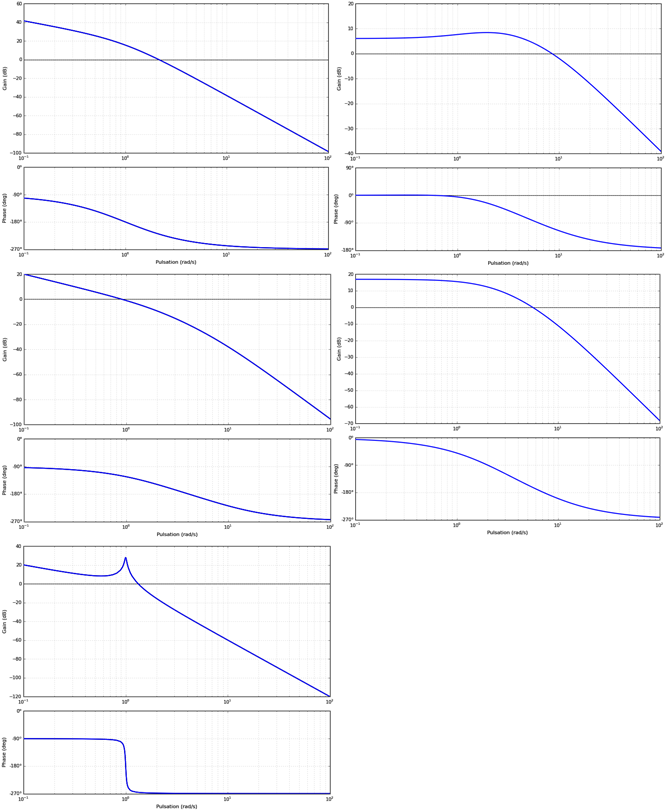
\includegraphics[width=.9\linewidth]{fig_01}
\end{center}

\subparagraph{}
\textit{Exprimer $\varepsilon(p)$ en fonction de $E(p)$ et $P(p)$.}

\subparagraph{}
\textit{Évaluer la valeur finale de $\varepsilon(t)$ lorsque $E(p)$ est un échelon d'amplitude $E_0$ et $P(p)$ est un échelon d'amplitude $P_0$.}


\subparagraph{}
\textit{Évaluer la valeur finale de $\varepsilon(t)$ lorsque $E(p)$ est un échelon d'amplitude $E_0$ et $P(p)$ est une rampe de pente $P_0$.}


\subparagraph{}
\textit{Évaluer la valeur finale de $\varepsilon(t)$ lorsque $E(p)$ est une rampe de pente $E_0$ et $P(p)$ est un échelon d'amplitude $P_0$.}


\subparagraph{}
\textit{Évaluer la valeur finale de $\varepsilon(t)$ lorsque $E(p)$ est une rampe de pente $E_0$ et $P(p)$est une rampe de pente  $P_0$.}
